\documentclass[UROP.tex]{subfiles}
\begin{document}

\bigskip
\section{\Large Methods}
\subsection{Antenna Design}
	The antenna will consist of 16 elements, arranged in two separate 8 element rings, one above the other.  Each element is a "bowtie" dipole, oriented in the vertical position to provide a vertically polarized field.  The drone is equipped with an ordinary dipole, also oriented in the vertical position so it can receive these fields.  
	
	\begin{figure}[H]
		\centering
		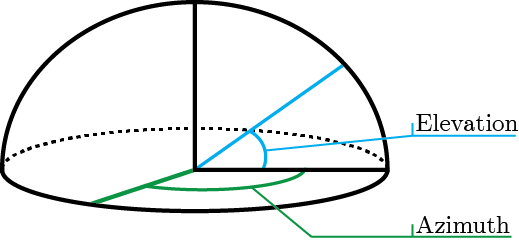
\includegraphics[]{elevation_azimuth.png}
		\caption{ Depiction of Azimuth and Elevation \label{fig:elevation_azimuth}}
	\end{figure}
	
	A dual ring phased array design will allow for more control in elevation.  The second, higher ring also creates more power at lower elevations.  The drone can and will fly at distances 20 miles away, at heights of 200 meters, so low elevation power is needed.  The design will also have 360$^{\circ}$ of azimuth.  A depiction of elevation compared to azimuth can be seen in Fig.~\ref{fig:elevation_azimuth}. \\
	
	In order to provide more power and less element coupling, a cylindrical ground plane is proposed to be placed in the center of the elements. This ground plane will reflect the power of the antenna elements facing the drone, and will give the option to turn off the other elements.\\
	
	Antenna simulations will and are currently being done in FEKO and HFSS to determine optimal element configurations.
\subsection{Phased Array Control System}
	Controlling the direction of requires changing the phase and amplitude of each antenna array element.  The elements will be initially fed with the same signal, but then attenuated and/or phase shifted to steer the beam towards the drone.  \\
	
	The control system will be managed by an STM processor.  This processor will be in charge of outputting correct phases and amplitudes to the phased array elements.  Calculations to determine the correct phase and amplitude values to steer the beam require rigorous testing and analysis.  Formulas exist for ideal isotropic antenna elements to determine phase and amplitude values, however this new design requires more intensive research to create accurate formulas.  During antenna simulations, methods will be constructed to help provide guidance to the control system in order to steer the beam correctly. \\
	

\end{document}
